\chapter{Refactoring spreadsheets}
\label{chapter:implementingrefactorings}

\noindent
\begin{figure}[h!]
\hspace*{0.003\textwidth}
\begin{subfigure}[c]{0.1\textwidth}
\f{=1+2+3}
\end{subfigure}
\begin{subfigure}[c]{0.1\textwidth}
$\xrightarrow{Parsing}$
\end{subfigure}
\fbox{
\begin{subfigure}[c]{0.15\textwidth}
\begin{tikzpicture}[-latex ,auto ,node distance =1.3 cm and 0.5cm ,on grid , semithick,
,
state/.style ={ circle ,top color =white ,
draw, minimum width =0.75 cm}]
\node[state] (RootPlus) {$+$};
\node[state] (SecondPlus) [below right=of RootPlus] {$+$};
\node[state] (Input1) [below left=of RootPlus] {1};
\node[state] (Input2) [below left=of SecondPlus] {2};
\node[state] (Input3) [below right=of SecondPlus] {3};

\path (RootPlus) edge node {} (Input1);
\path (RootPlus) edge node {} (SecondPlus);
\path (SecondPlus) edge node {} (Input2);
\path (SecondPlus) edge node {} (Input3);
\end{tikzpicture}
\end{subfigure}
\begin{subfigure}[c]{0.14\textwidth}
$\xrightarrow{Refactoring}$
\end{subfigure}
\begin{subfigure}[c]{0.17\textwidth}
\begin{tikzpicture}[-latex ,auto ,node distance =1.3 cm and 0.5cm ,on grid , semithick,
,
state/.style ={ circle ,top color =white ,
draw, minimum width =0.75 cm}]
\node[state] (Root) {$F$};
\node[state] (11) [below left=of Root] {\tiny{\f{SUM}}};
\node[state] (12) [below right=of Root] {[]};
\node[state, node distance = 1.3cm and 0.85cm] (21) [below left =of 12] {1};
\node[state, node distance = 1.32cm and 0.85cm] (22) [below =of 12] {2};
\node[state, node distance = 1.3cm and 0.85cm] (23) [below right=of 12] {3};

\path (Root) edge node {} (11);
\path (Root) edge node {} (12);
\path (12) edge node {} (21);
\path (12) edge node {} (22);
\path (12) edge node {} (23);
\end{tikzpicture}
\end{subfigure}
}
\begin{subfigure}[c]{0.1\textwidth}
$\xrightarrow{Printing}$
\end{subfigure}
\begin{subfigure}[c]{0.145\textwidth}
\f{=SUM(1,2,3)}
\end{subfigure}
\caption{This chapter details the AST to AST transformations that implement the refactorings.}
\end{figure}

Refactoring a spreadsheet involves changing the sheets, cells and formulas in a workbook in such a way that the desired change is performed.
Excel provides an API to change the worksheet and cells, and most other elements of a workbook.
When it is desired to refactor formulas this means the original formula string must be changed into a new formula string.
This is usually implemented by parsing the formula, performing the desired transformations on the AST and then printing the AST back to a string form \cite{fowler1999refactoring}.
The inner workings of the parser are described in \ref{chapter:parsing}.
This Chapter covers how the AST is transformed for each refactoring and how it is printed.

The refactorings were implemented in the BumbleBee Excel Add-In, and presented to the user through a context menu as seen in Figure X.
This context-menu automatically determines if a refactoring can be performed on the specific selected cell(s) and disables inapplicable refactorings.
\todo{Screenshot van het bumblebee refactoring context-menu}

It must be noted that all refactorings have a major deficiency: they cannot be undone.
The reason for this is a technical limitation imposed by Excel: the Excel undo-redo stack is not available to Excel Add-Ins.
Instead as soon as a Excel Add-In changes the Excel spreadsheet file, in fact as soon as it interacts with the internal document model even if it does not change anything, the Excel undo-redo stack gets cleared.
There is a fairly complicated way to work around this\footnote{Visual Basic for Application macros do have access to the undo-redo stack. Thus theoretically one could insert a VBA macro which saves the cells to be altered to the stack. However this has the major disadvantage of changing every spreadsheet file touched to a macro-enabled spreadsheet file and leaving a macro behind.}, this was deemed outside of the scope of this thesis.
As long as Excel keeps this limitation this will always be a severe limitation to any tool that automatically changes spreadsheet files for the user.

\section{\rf{Extract formula}}

The \rf{extract formula} refactoring is analogous to the \rf{extract method} (object oriented programming) or \rf{extract function} (functional programming) refactorings, and also to the \rf{extract local variable} refactoring.
All have in common that one takes a collections of composable units, removes these from the parent unit and places them into a new parent unit of the same type:

\begin{tabular}{@{}lll@{}}
	\toprule
	Refactoring & Composable unit & Parent unit \\
	\midrule
	Extract Method & Statements & Method \\
	Extract Function (Functional) & Expression & Function \\
	Extract Function (Imperative) & Statements & Function \\
	Extract local variable & Expression & Variable \\
	\textbf{Extract formula} & Expression & Formula \\
	\bottomrule
\end{tabular}

The goal of the \rf{extract formula} refactoring is to move part of a formula expression, a sub-formula, to another cell, which has the following potential advantages:

\begin{enumerate}
\item Remove "magic numbers" or other constants and make them easy to adjust.
\item Make a formula easier to understand by splitting it into more smaller components.
\item Reduce duplication in a formula by extracting common sub-formulas into another cell.
\end{enumerate}

\subsection{User interface}

\begin{figure}
\begin{minipage}[c][8cm][c]{0.5\textwidth}
\centering
\vspace*{\fill}
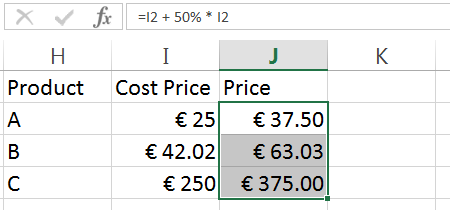
\includegraphics[height=3cm]{implementation/extractformula/21}
\subcaption{User selects cells to be refactored}
\label{fig:extractformulaexample2a}

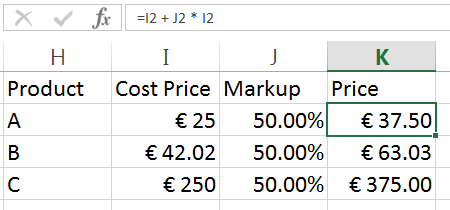
\includegraphics[height=3cm]{implementation/extractformula/23}
\addtocounter{subfigure}{1}
\subcaption{Refactoring has been performed}
\label{fig:extractformulaexample2c}
\end{minipage}
\begin{minipage}[c][8cm][t]{0.5\textwidth}
\vspace*{\fill}
\centering
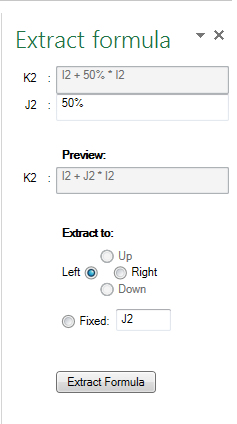
\includegraphics[height=7cm]{implementation/extractformula/22}
\addtocounter{subfigure}{-2}
\subcaption{User selects subformula to be extracted}
\label{fig:extractformulaexample2b}
\end{minipage}
\caption{An example application of \rf{Extract Formula}}
\label{fig:extractformulaexample2}
\end{figure}

The refactoring requires the user to select cell(s) to be refactored, type in the subformula to be extracted and select where the extraction should occur to.
Figure \ref{fig:extractformulaexample2} shows the process as experienced by the user.
The user first selects the formulas to be extracted (Figure \ref{fig:extractformulaexample2a}) and clicks the Extract Formula entry in the refactoring context menu (not shown).
A side-panel pops out which allows the user to enter the sub-formula to be extracted and where it should be extracted to (Figure \ref{fig:extractformulaexample2b}) and presses the Extract Formula button.
In the example the \f{50\%} subformula was extracted to the left, and Figure \ref{fig:extractformulaexample2c} shows the situation after the user has named the new column.

\subsection{Implementation}

The implementation consists of 2 parts.
The first part handles actual placement of the formula in the cells and the moving if neccesary, the second part operates solely on the formula and refactors it to the desired form.

\subsubsection{Formula Refactoring}

Call the original formula $F_{or}$, the refactored formula $F_{new}$, the (user-supplied) subformula to be extracted $F_{search}$.
The spreadsheet refactoring code also provides the target $F_{search}$ will be moved to as $F_{repl}$.
The refactoring works by first parsing all formulas to AST.
Then $AST_{or}$ is walked through and every occurrence of $AST_{search}$ is replaced by $AST_{repl}$, yielding $AST_{new}$, this is illustrated in Figure \ref{fig:extractformulaASTtransformations}.
$AST_{new}$ is then printed to $F_{new}$, which is returned.
The C\# code for the AST replacement can be found in Listing \ref{lst:astreplace}.

You might have noticed that the AST transformation is somewhat similar to the BumbleBee formula transformation rules.
However, it is complimentary rather than identical.
We could have tried to written this transformation as a BumbleBee rule "\f{=I2 + [a] * I2}".
However, BumbleBee would have searched for the "outer" formula, keeping the \f{[a]} $\gets$ \f{50\%} available for the replacement rule.
In contrast, this transformation searches for the \f{[a]} "inner" formula, and replaces it with something different.

\begin{figure}
\centering
{
\begin{subfigure}[t]{0.12\textwidth}
\centering
\begin{tikzpicture}[-latex ,auto ,node distance =1.3 cm and 0.5cm ,on grid , semithick,
,
state/.style ={ circle ,top color =white ,
draw, minimum width =0.75 cm}]
\node[state] (Percent) {\tiny \%};
\node[state] (Constant50) [below =of Percent] {\tiny 50};

\path (Percent) edge node {} (Constant50);
\end{tikzpicture}
\caption*{${\scriptscriptstyle AST_{search}}$}
\end{subfigure}
}
{
\begin{subfigure}[t]{0.24\textwidth}
\centering
\begin{tikzpicture}[-latex ,auto ,node distance =1.3 cm and 0.8cm ,on grid , semithick,
,
state/.style ={ circle ,top color =white ,
draw, minimum width =0.75 cm}
,
redstate/.style ={ circle , fill=red,
draw, minimum width =0.75 cm}]
\node[state] (OpPlus) {$+$};
\node[state] (OpMult) [below right =of OpPlus] {$\ast$};

\node[state] (RefI2) [below left =of OpPlus] {\tiny Ref};
\node[state] (ConstI2) [below =of RefI2] {\tiny \f{I2}};

\path (RefI2) edge node {} (ConstI2);

\node[state] (RefI22) [below right = 1.3cm and 0.52cm of OpMult] {\tiny Ref};
\node[state] (ConstI22) [below =of RefI22] {\tiny \f{I2}};

\path (RefI22) edge node {} (ConstI22);

\node[redstate] (Percent) [below left = 1.3cm and 0.42cm of OpMult] {\tiny \%};
\node[redstate] (Constant50) [below =of Percent] {\tiny 50};

\path (Percent) edge node {} (Constant50);

\path (OpPlus) edge node {} (OpMult);
\path (OpPlus) edge node {} (RefI2);
\path (OpMult) edge node {} (RefI22);
\path (OpMult) edge node {} (Percent);
\end{tikzpicture}
\caption*{${\scriptscriptstyle AST_{or}}$}
\end{subfigure}
}
{
\begin{subfigure}[t]{0.12\textwidth}
\centering
\begin{tikzpicture}[-latex ,auto ,node distance =1.3 cm and 0.5cm ,on grid , semithick,
,
state/.style ={ circle ,top color =white ,
draw, minimum width =0.75 cm}]
\node[state] (RefJ2) {\tiny Ref};
\node[state] (ConstJ2) [below =of RefJ2] {\tiny \f{J2}};

\path (RefJ2) edge node {} (ConstJ2);
\end{tikzpicture}
\caption*{${\scriptscriptstyle AST_{repl}}$}
\end{subfigure}
}
{
\begin{subfigure}[b]{0.1\textwidth}
\centering
\vspace*{4em}
$\xrightarrow[Returns]{}$
\vspace*{2em}
\end{subfigure}
}
{
\begin{subfigure}[t]{0.24\textwidth}
\centering
\begin{tikzpicture}[-latex ,auto ,node distance =1.3 cm and 0.8cm ,on grid , semithick,
,
state/.style ={ circle ,top color =white ,
draw, minimum width =0.75 cm}
,
greenstate/.style ={ circle , fill=green,
draw, minimum width =0.75 cm}]
\node[state] (OpPlus) {$+$};
\node[state] (OpMult) [below right =of OpPlus] {$\ast$};

\node[state] (RefI2) [below left =of OpPlus] {\tiny Ref};
\node[state] (ConstI2) [below =of RefI2] {\tiny \f{I2}};

\path (RefI2) edge node {} (ConstI2);

\node[state] (RefI22) [below right = 1.3cm and 0.52cm of OpMult] {\tiny Ref};
\node[state] (ConstI22) [below =of RefI22] {\tiny \f{I2}};

\path (RefI22) edge node {} (ConstI22);

\node[greenstate] (RefJ2) [below left = 1.3cm and 0.42cm of OpMult] {\tiny Ref};
\node[greenstate] (ConstJ2) [below =of RefJ2] {\tiny \f{J2}};

\path (RefJ2) edge node {} (ConstJ2);

\path (OpPlus) edge node {} (OpMult);
\path (OpPlus) edge node {} (RefI2);
\path (OpMult) edge node {} (RefI22);
\path (OpMult) edge node {} (Percent);
\end{tikzpicture}
\caption*{${\scriptscriptstyle AST_{new}}$}
\end{subfigure}
}
\caption{AST transformation to implement extract formula refactoring}
\label{fig:extractformulaASTtransformations}
\end{figure}

\subsubsection{Spreadsheet refactoring}

\todo{Dit moet nog iets duidelijker.}

The spreadsheet refactoring differs slightly depending on if the subformula get to a single cell or if the extraction occurs in a direction.
If to a single cell, that cell gets assigned the subformula.
Otherwise new cells are created in the appropriate direction and they get assigned the subformula.

The AST replacement is then performed on the original formula, and the new formula is assigned to the cell that needs to be refactored.
If multiple cells are refactored at once, the above process is performed for all of them.
Formulas with the same R1C1 $F_{or}$ have the same R1C1 $F_{new}$ so the output of the formula refactoring is cached.

The C\# code for the spreadsheet refactoring can be found in Listing \ref{lst:extractformula}.

\subsection{Detection of applicability}

Extract formula is always applicable to a formula cell, as even a very simple formula like \f{=1} still has a component that can be extracted.
In this case if \f{=1} would be extracted to \f{A1} the original cell would become \f{=A1}.
Of course, whether it is a good thing to perform this refactoring is dubious, but BumbleBee relies on the user to make this assessment.

\subsection{Improvements over RefBook \rf{Extract row or column} and \rf{Extract Literal}}
\label{subsubsec:improvementsextractformula}

Two specialized versions of this refactorings where previously described by Bamade and Dig \cite{badame2012refactoring} and implemented in their RefBook tool.
Refbooks \rf{Extract Row or column} and \rf{Extract Literal} refactorings can both be performed by \rf{Extract formula}.

The author has chosen to not keep the \rf{extract row or column} refactoring name because it does not fully describe the refactoring, a full row or column does not necessarily have to be extracted, and to keep the name in line with refactoring names in other domains.

The RefBook \rf{extract literal} refactoring can put a constant value into a cell and replace the occurrences of it with references to that cell, this can also be achieved with the BumbleBee \rf{extract formula} refactoring.
In addition this is possible for any constant expression, an expression without references, instead of only for constants.

The BumbleBee \rf{Extract Formula} refactoring has several advantages over Badame's implementation of \rf{Extract row or column}.
Firstly RefBook does not handle operator precedence.
This can be very problematic for this refactoring and in the authors opinion should prevent is from being implemented, because one of the prime properties of a refactoring should be that it does not change the program results.
Note that the RefBook authors were aware of this deficiency, and left this as future work.
This future work has been performed by the thesis author.

Secondly RefBook can only handle a single row or column, which has to have exactly the same R1C1 formula. It can only extract the subformula to a column right of or row up of the original range.
BumbleBee can handle arbitrarily shaped ranges, with the only requirement that the subformula to be extracted occurs in all selected formulas.
Furthermore in addition to extracting to a cell neighboring the original formula cell (up, down, left or right) it can also extract the subformula to a single shared cell location.
This is very useful to remove duplication and makes the refactoring more universal by merging the \rf{extract literal} refactoring into it.

\section{\rf{Inline formula}}

\section{\rf{Introduce (Conditional) Aggregate}}

\section{\rf{Group References}}

\section{\rf{Fixate References}}

\todo{Unsure of ik deze nog wil implementeren, maar lijkt zeer laaghangend fruit.}

The Fixate References is similar to the \rf{Make Cell Constant} refactoring described by Badame \cite{badame2012refactoring}.
Maar beter want: user kan zelf selecteren welke cellen wel/niet absolute.

"Fixate references" beschrijft 100x beter wat de refactoring doet dan "Make cell constant". "Make cell constant" zou eerder impliceren dat je het resultaat van de cell berekening neemt en dat opslaat i.p.v. de formula. Wat trouwens ook weer een potentiele refactoring is, maar misschien een beetje een anti-pattern in excel.

\section{\rf{Introduce name}}

\todo{Kandidaat voor implementatie, meer laaghanged fruit.}

Cell (of range?) een naam geven, overal waar die naar gereferenced wordt vervangen door cell naam.
Of gelijk bij extract formula intregrereren!